\chapter{TEST GENERATION}
\label{chapter:test_generation}

\section{Test Generation with Graphwalker}
\par
Graphwalkers provides multiple ways for test generation from models. The general pattern for test selection criterion can be observed in figure \ref{Fig:raphwalker_testselection_example}.

\begin{figure} [htbp!]
	\centering
					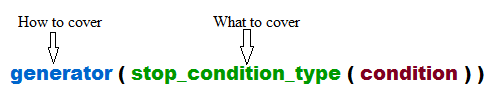
\includegraphics[width=1\textwidth]{figures/Graphwalker_testselection_example.png}
					\caption{\label{Fig:raphwalker_testselection_example} Graphwalker Test Selection pattern}
\end{figure}
\par
As reader can observe, selection criterion consists of generator, stop condition type and condition. Generator stands for the coverage algorithm which takes stop condition type as a parameter. Stop condition type gives Graphwalker information about what exactly to cover using the coverage algorithm. Condition might vary depending on stop condition type.

\subsection{Generator Algorithms}
\par
One of the generator algorithms in Graphwalker is random. This is the algorithm which will be used most extensively for test generation in this thesis. It is also known with name Drunkard's walk or Random walk. This algorithm selects edges not blocked by guards coming out of vertex completely randomly during traversal and continues doing same until stop condition is met. As a parameter it can take multiple stop conditions such as edge or vertex coverage. Examples of its usage can be observed below. 
\begin{lstlisting}
random(vertex_coverage(100))
random(never)
random(reached_vertex(v_SomeVertex))
random(reached_vertex(v_SomeVertex) and edge_coverage(100))
random((reached_vertex(v_SomeVertex) and vertex_coverage(100)) || time_duration(500))
\end{lstlisting}

\par
Weighted\_random coverage does exactly same as random algorithm, but takes into consideration weight annotations on edge labels and decides on next edge based on these weights. Basically, higher the edge weight, more likely it is that Graphwalker will take that edge when its source vertex is reached. It is extremely useful when company has usage profiles of application from customers, so they can test more extensively features which are used more often. Example usage of it would be also same as in case of random, but instead of random keyword we use weighted\_random.

\par
Quick-random tries to cover model with the shortest path. It marks already taken edges 
as visited and tries not to take them any more if there is other option available. Problem is that it does not work with \acrshort{efsm} and might take an edge which is blocked by guard. That is the reason why it cannot be used in our case as most of edges in our models are annotated with guards. Example usage would look exactly same as random but with the keyword quick\_random.

\par
A\_Star algorithm can be used for generating shortest path to an edge or vertex in model. In this case passed stop condition needs to specify which edge or vertex needs to be reached. The example usage can be found below.

\begin{lstlisting}
a_star(reached_edge(e_SomeEdge))
a_star(reached_vertex(v_SomeVertex))
\end{lstlisting}

\subsection{Stop Conditions}
\par
Edge and vertex coverage are the most used stop conditions for any type of random algorithm. They take as a parameter integer which stands for percentage. So, random(edge\_coverage(95)) would mean that Graphwalker can stop only after it covers 95\% of the edges.

\par
Reached vertex stop condition

\section{Layers}
\section{Minimal Required Path}
\subsection{Graphwalker GUI} 


\begin{lstlisting}
http://localhost:4200/camera
http://localhost:4200/camera/<id>
http://localhost:4200/instruction
http://localhost:4200/instruction/<id>
\end{lstlisting}